\chapter{Experimentos}
\label{chap:experimetos}
Para probar la metodología expuesta en el capitulo anterior se realizaron varios experimentos que hemos dividido en dos partes: una con experimentos visuales sobre datos obtenidos de tomógrafos y la segunda parte con experimentos numéricos sobre modelos analíticos. Para todos nuestros experimentos hemos asumido, sin perdida de generalidad, que tenemos volúmenes discretizados $G_{1}$ (en otras palabras $\Delta = 1$). Por lo tanto hemos escalado los blobs de la Sección \ref{sec:repImplicita} de manera consistente (por ejemplo, para el blob diseñado para la rejilla \emph{bcc} el radio es escalado por $\frac{1}{\sqrt{2}}$).

Para la visualización de todas las mallas hemos utilizado el API gráfico OpenGL\texttrademark \cite{openGLSite} la cual permite iluminar con el modelo de Phong \eqref{ec:phongModelo} pero utiliza para sombrear el modelo de Gouraud \eqref{ec:gouraudShading} \cite{redBook}. El software utiliza una luz direccional, ver Sección \ref{sec:visualizarMallas} cuya componente ambiental es igual a cero y sus otros dos componentes son de color blanco. La dirección de dicha luz es paralela al vector perpendicular al plano de proyección y tiene un sentido opuesto al observador.

Las propiedades del material son constantes en todos los casos y se proporciona en la Tabla \ref{table:material} en relación al modelo de iluminación \eqref{ec:phongModelunaLuz}. 

\begin{table}[htp]
\begin{center}
  \begin{tabular}{|c|c|c|c|}
    \hline
    $\rho_a$ & $\rho_d$ & $\rho_s$ & $\gamma$ \\
    \hline
    $(0.7, 0.7, 0)$ & $(0.9, 0.9, 0)$ & $(0, 0, 0)$ & $1$  \\
    \hline
  \end{tabular}
\end{center}
\caption[Propiedades del material con el que se visualizan las mallas]{Propiedades del material con el que se visualizan las mallas. Estos valores se usan en el modelo de iluminación \eqref{ec:phongModelunaLuz}}
\label{table:material}
\end{table}

%Siguiendo la metodología expuesta en el capitulo anterior se realizaron algunos experimentos. Los experimentos se pueden clasificar en dos tipos. Primero en algunos conjuntos de datos provenientes de reconstrucciones tomográficas. En este tipo de datos la selección de un isovalor $\tau$ para extraer una superficie fue hecha de manera arbitraria seleccionando aquel que produce superficies interesantes. Las comparaciones se hacen usando el mismo valor $\tau$ para ambos algoritmos.

%En la segunda parte se hace uso de maquetas. Se cuenta con SW capaz de reconstruir un volumen $v$ a partir de la descripción geométrica de un objeto por medio de algún método de reconstrucción. Los volúmenes $v$ producidos artificialmente se les llama \emph{phantoms}. La ventaja de estas maquetas es que dado que contamos con la descripción de los objetos conocemos de alguna manera la superficie correcta descrita por \eqref{ec:isosupeficie} y por lo tanto si hacemos una buena umbralización $\mathcal{A}_{\tau}$ puede coincidir con $S_{\tau}$ los suficiente como para que podamos medir la calidad del conjunto de normales arrojado por nuestro método sobre $\mathcal{A}_{\tau}$ comparándolo con aquellas de $S_{\tau}$.

%Durante este capítulo se tomo la convención de utilizar una clave de colores para distinguir las diferentes visualizaciones. De esta manera una superficie de color amarillo representa una superficie obtenida por MC, una superficie color verde representa una superficie obtenida con Artzy y cuyas normales son aquellas producidas mediante la orientación geométrica de sus caras. Finalmente una superficie color naranja representa una superficie obtenida por Artzy cuyas normales fueron ponderadas con el método expuesto en el capitulo anterior. Aun así todas las imágenes han sido debidamente etiquetadas y se describen en cada sección los parámetros completos con los que fueron producidas.

%También se hace la aclaración que el blob fue escalado adecuadamente para nuestra implementación de Artzy donde la rejilla es $G_{1}$ y por lo tanto el blob usado para el caso de \emph{bcc} (o \emph{fcc}) es: $b(m = 2, \alpha = 13.36, a = 3.394213972)$ donde la $a$ obtenida en el capítulo anterior ha sido multiplicada por $\sqrt{2}$.

\section{Experimentos visuales}
\label{sec:experimentosVisuales}

Para los primeros experimentos utilizamos conjuntos de datos disponibles en varios sitios públicos, por ejemplo de \cite{volumeLibrary}. Estos conjuntos de datos han sido obtenidos por medio de TAC pero desconocemos el método usado para la obtención de la aproximación $v_{G_{\Delta}}$ (los TAC usan métodos de aproximación y muestreo conocidos como reconstrucción por medio de proyecciones \cite{tomografyBook}). Por lo tanto desconocemos las funciones originales y nuestras comparaciones son puramente visuales.

%Para los experimentos se ha hecho uso del modelo de Phong \eqref{ec:phongModelo} junto con sombreado de Gouraud \eqref{ec:gouraudShading}. Como se explico en las secciones correspondientes. Esto requiere de definir un conjunto de parámetros. La luz en todos los casos es una fuente de luz direccional cuyos componentes especular y ambiental son de color blanco y cuya componente ambiental es negra y no hay iluminación ambiental global. La dirección de la luz es normal al plano de proyección y su sentido es desde el espectador al centro de la escena.

%Para el algoritmo de Artzy la superficie representada en color verde. Las propiedades de los materiales, en relación a lo expuesto en el modelo de iluminación de Phong se resumen en la siguiente tabla:

% \begin{center}
%   \begin{tabular}{|l|r|r|r|r|r|}
%     \hline
%     Malla & $\rho_a$ & $\rho_d$ & $\rho_s$ & $\gamma$ \\ 
%     \hline
%     Marching Cubes & $\langle 0.7, 0.7, 0 \rangle$ & $\langle 0.9, 0.9, 0 \rangle$ & $\langle 0.9, 0.9, 0 \rangle$ & $0.5$ \\
%     Artzy & $\langle 0, 0.5, 0 \rangle$ & $\langle 0.53, 1, 0\rangle$ & $\langle 0, 1, 0 \rangle$ & $128$  \\
%     Artzy con ponderación de normales & $\langle 0.48, 0.14, 0 \rangle$ & $\langle 0.96, 0.29, 0 \rangle$ & $\langle 0.48, 0.14, 0 \rangle$ & $128$  \\
%     \hline
%   \end{tabular}
% \end{center}

%Las figuras siguientes muestra cada malla, vista desde el mismo ángulo y a la misma distancia con las mismas condiciones de iluminación.

Primero usamos un conjuntos de datos con 324 de ancho, 301 de alto y 56 de profundidad que se obtiene de la reconstrucción de una langosta. Para este conjunto de datos usamos un umbral $\tau = 26$ seleccionado manualmente. En la figura \ref{fig:lobster1} es interesante notar que en las zonas donde la superficie es bastante uniforme el método de ponderación de normales no suaviza tanto como el MC.

\begin{figure}[htp]
  \begin{center}
    \subfigure[Malla de Artzy]{\label{fig:lobster1AZ}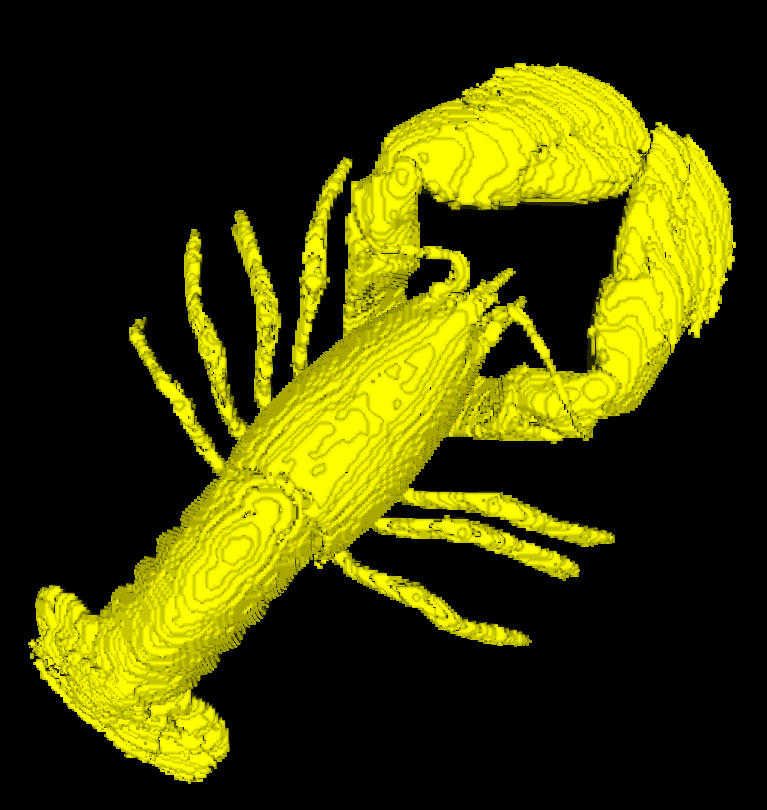
\includegraphics[scale=0.26]{img/cap03/Lobster32AZ2}}
    \subfigure[Malla de MC]{\label{fig:lobster1MC}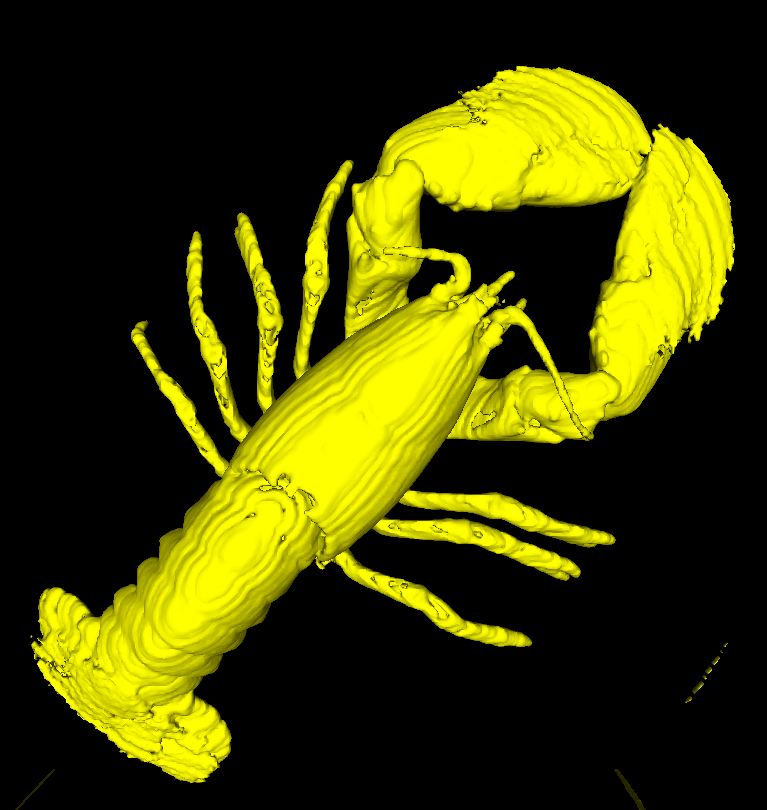
\includegraphics[scale=0.26]{img/cap03/Lobster32MC2}} \\
    \subfigure[Malla de Artzy con ponderación de normales caso \emph{sc}]{\label{fig:lobster1SC}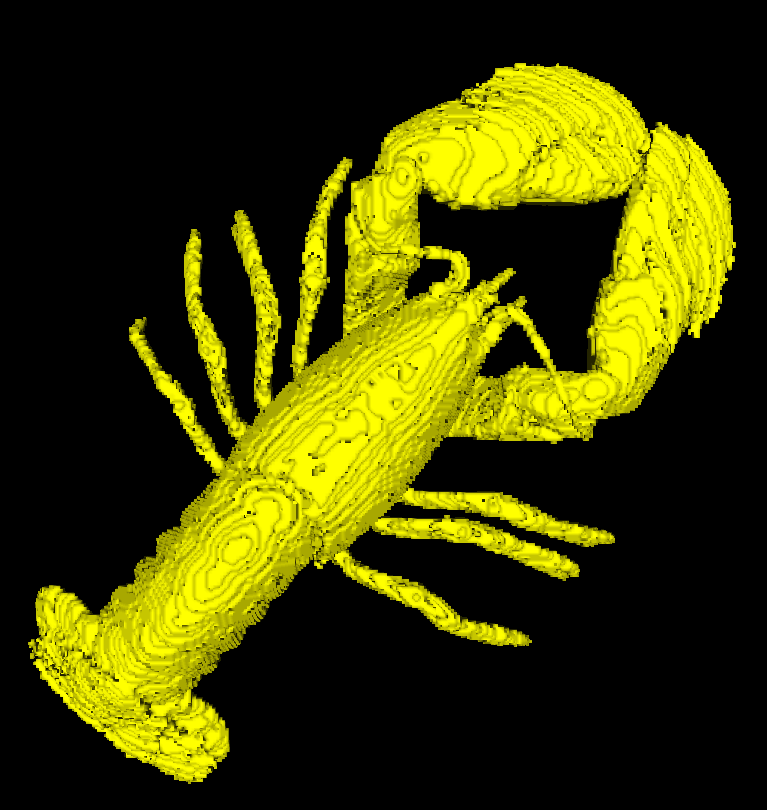
\includegraphics[scale=0.26]{img/cap03/Lobster32NS-SC2}}
    \subfigure[Malla de Artzy con ponderación de normales caso \emph{bcc}]{\label{fig:lobster1BCC}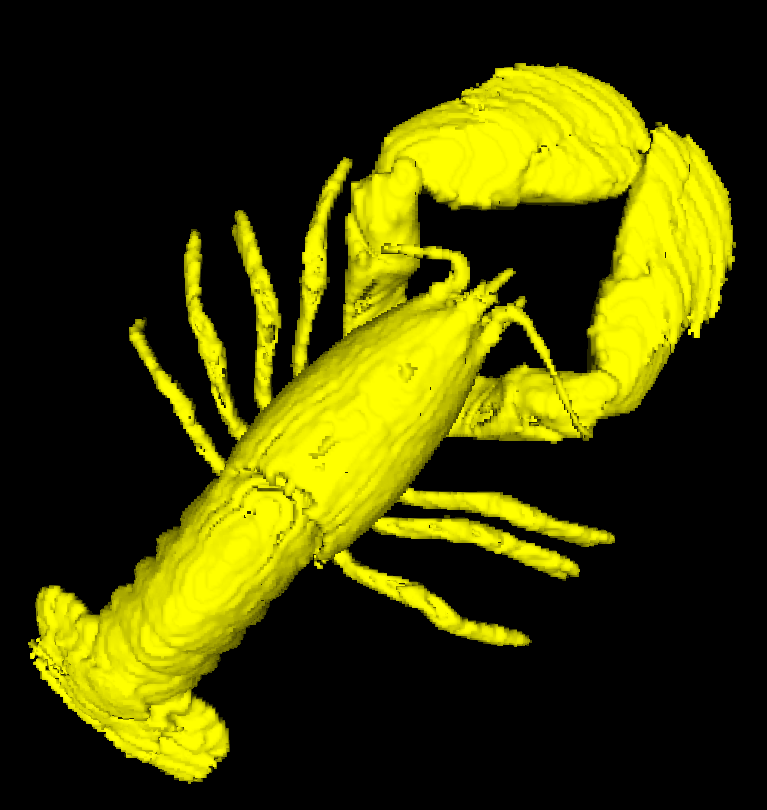
\includegraphics[scale=0.26]{img/cap03/Lobster32NS-BCC2}}
  \end{center}
  \caption[Comparación visual de superficies formadas a partir de la reconstrucción de una langosta]{Comparación visual de superficies formadas a partir de la reconstrucción de una langosta.}
  \label{fig:lobster1}
\end{figure}

En la Figura \ref{fig:lobster2} el conjunto de imágenes muestra una vista diferente de la misma superficie de la Figura \ref{fig:lobster1}. En esta vista queda de manifiesto que el método no suaviza demasiado en zonas donde la topología del modelo es compleja, es decir hace un buen trabajo pues no pierde detalles finos de la malla.

\begin{figure}[htp]
  \begin{center}
    \subfigure[Malla de Artzy]{\label{fig:lobster2AZ}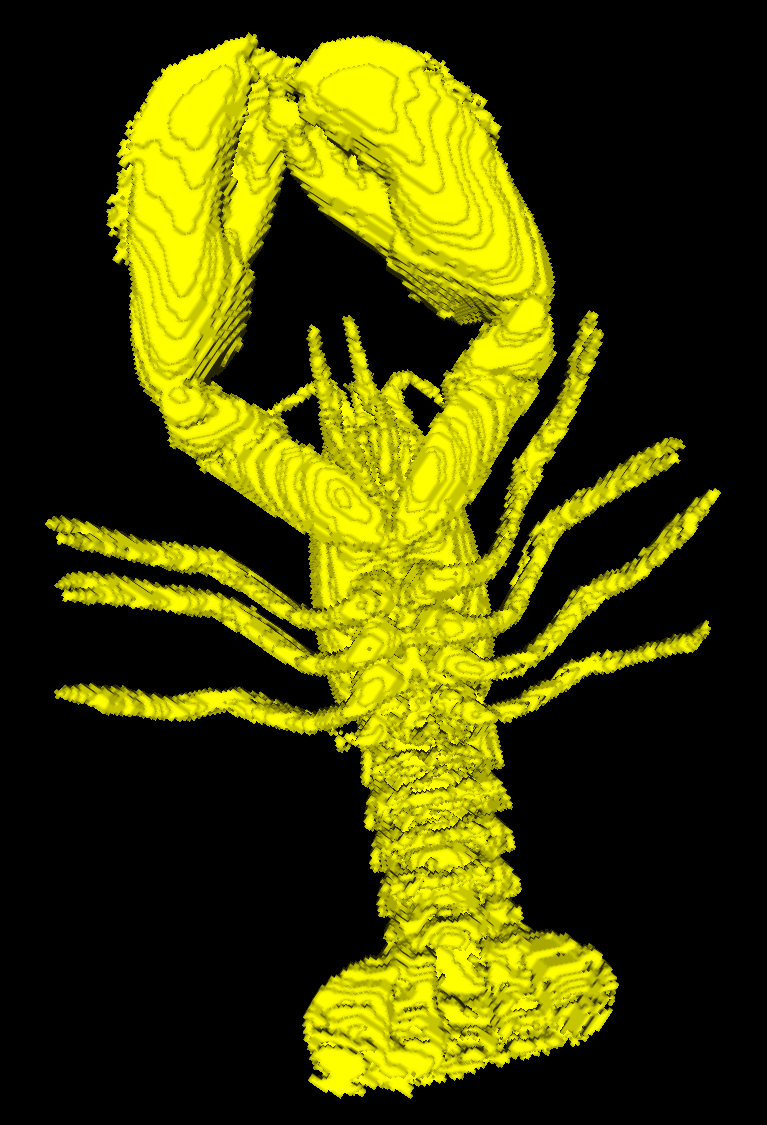
\includegraphics[scale=0.24]{img/cap03/Lobster32AZ1}} 
    \subfigure[Malla de MC]{\label{fig:lobster2MC}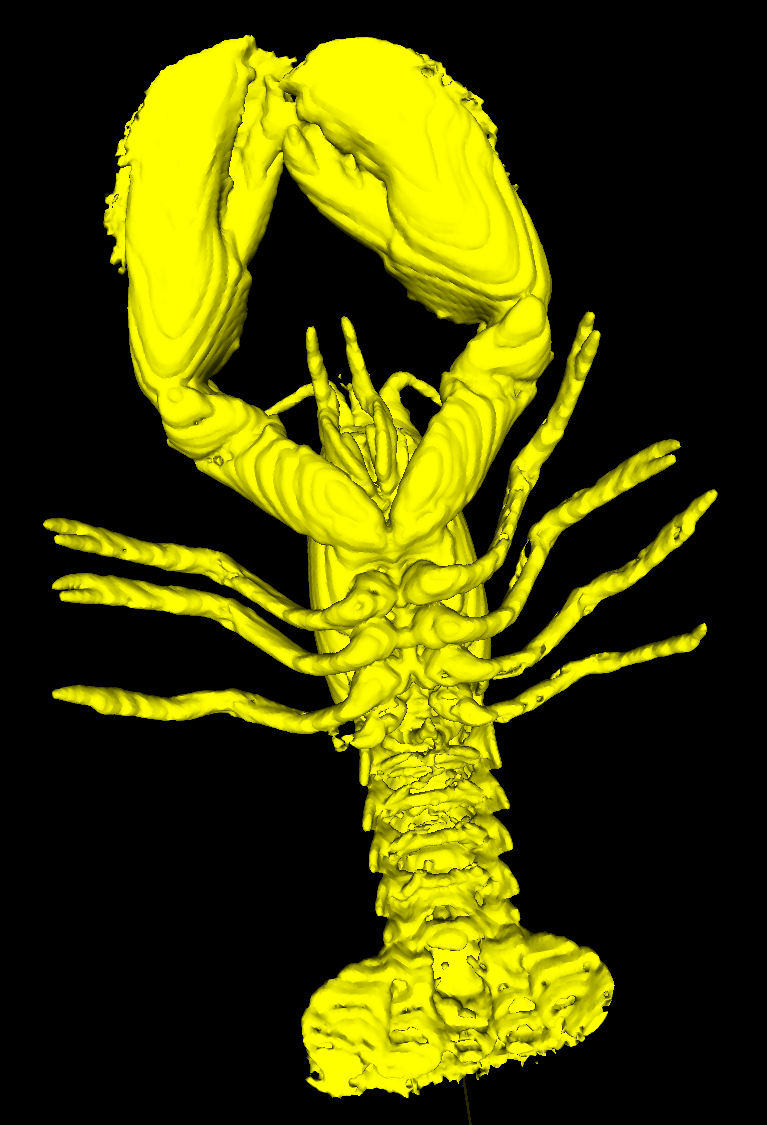
\includegraphics[scale=0.24]{img/cap03/Lobster32MC1}} \\
    \subfigure[Malla de Artzy con ponderación de normales caso \emph{sc}]{\label{fig:lobster2SC}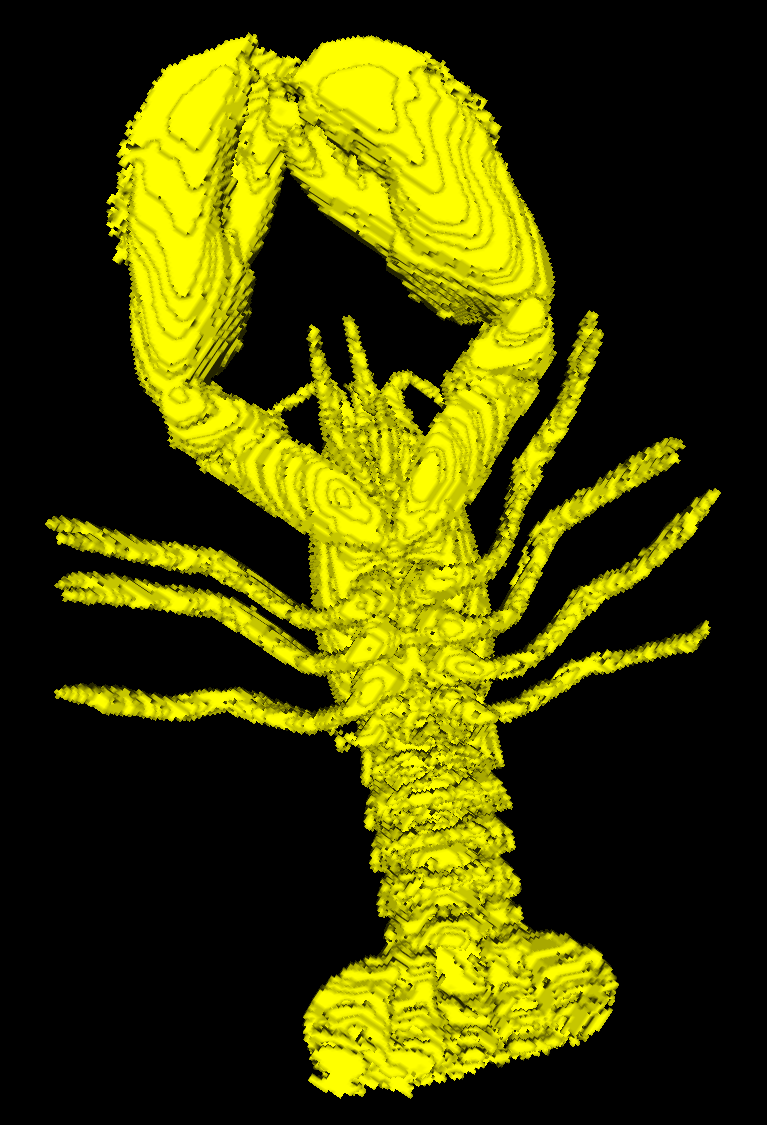
\includegraphics[scale=0.24]{img/cap03/Lobster32NS-SC1}} 
    \subfigure[Malla de Artzy con ponderación de normales caso \emph{bcc}]{\label{fig:lobster2BCC}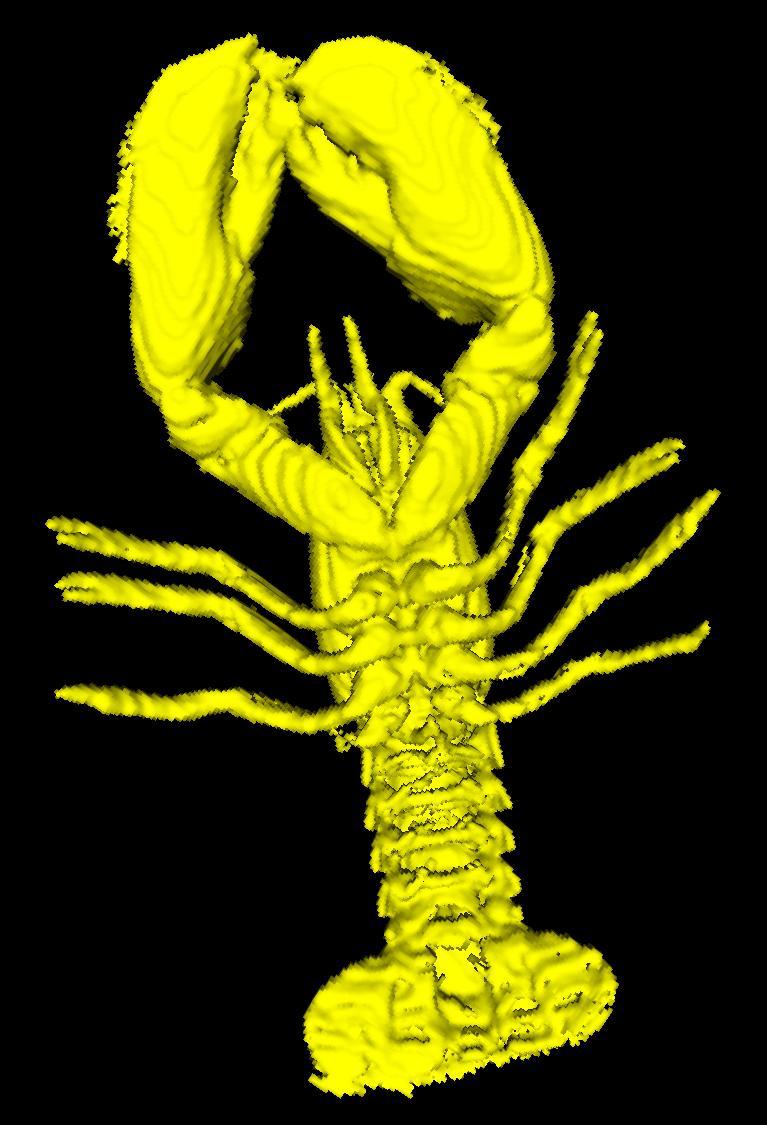
\includegraphics[scale=0.24]{img/cap03/Lobster32NS-BCC1}} \\
  \end{center}
  \caption[Comparación visual de superficies de la reconstrucción de una langosta. Son las mismas mallas que las de la Figura \ref{fig:lobster1} vistas desde otro punto de vista]{Comparación visual de superficies de la reconstrucción de una langosta. Son las mismas mallas que las de la Figura \ref{fig:lobster1} vistas desde otro punto de vista.}
  \label{fig:lobster2}
\end{figure}

El siguiente experimento visual fue hecho sobre un conjunto de datos de reconstrucción de una cabeza humana, con tamaño 256 en cada dimensión, en estos datos se seleccionó un umbral $\tau = 103$ que permite ver muchas zonas relativamente homogéneas. Se pueden ver los resultados en la Figura \ref{fig:MRI-Head}.

\begin{figure}[htp]
  \begin{center}
    \subfigure[Malla de Artzy]{\label{fig:MRI-HeadAZ}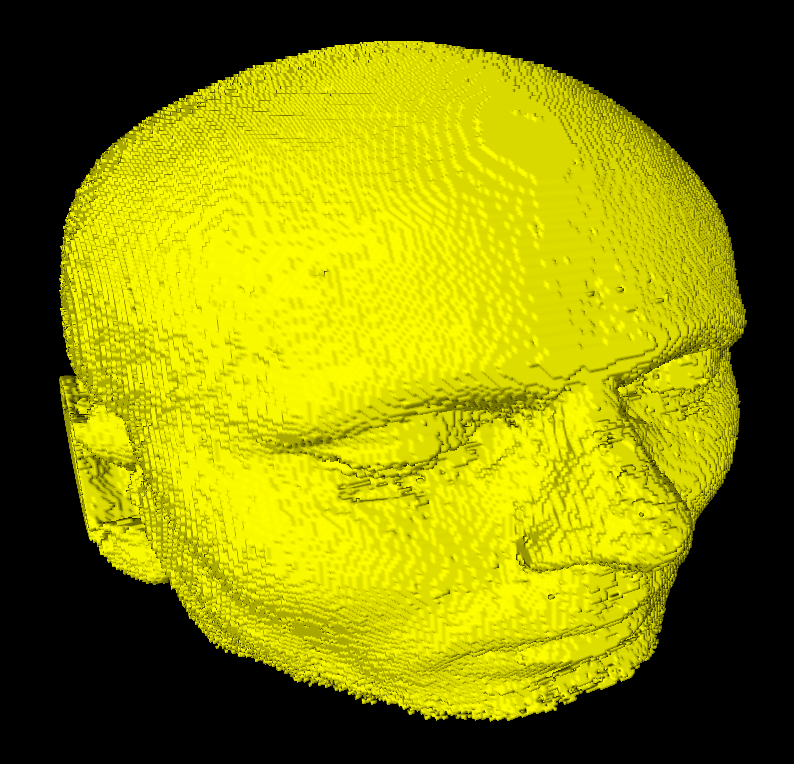
\includegraphics[scale=0.34]{img/cap03/MRI-Head-103-AZ}}
    \subfigure[Malla de MC]{\label{fig:MRI-HeadMC}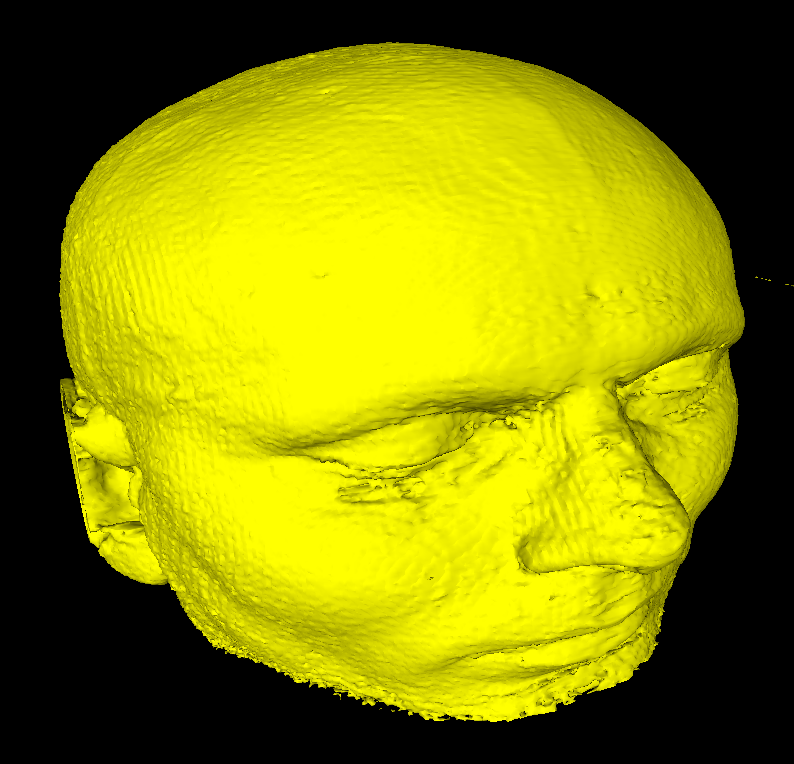
\includegraphics[scale=0.34]{img/cap03/MRI-Head-103-MC}} \\
    \subfigure[Malla de Artzy con ponderación de normales caso \emph{sc}]{\label{fig:MRI-HeadSC}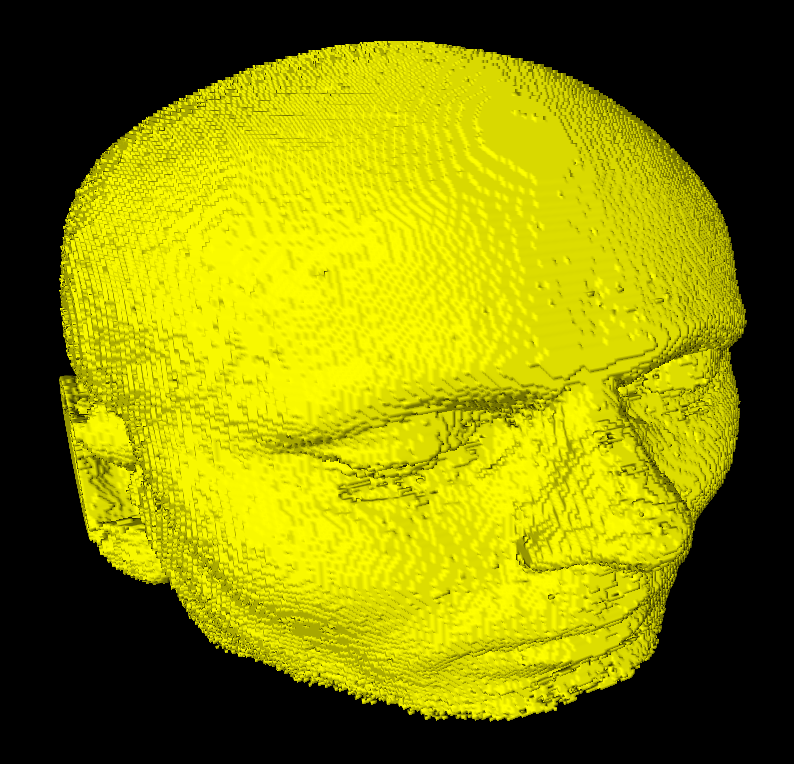
\includegraphics[scale=0.34]{img/cap03/MRI-Head-103-AZ-NS-SC}}
    \subfigure[Malla de Artzy con ponderación de normales caso \emph{bcc}]{\label{fig:MRI-HeadBCC}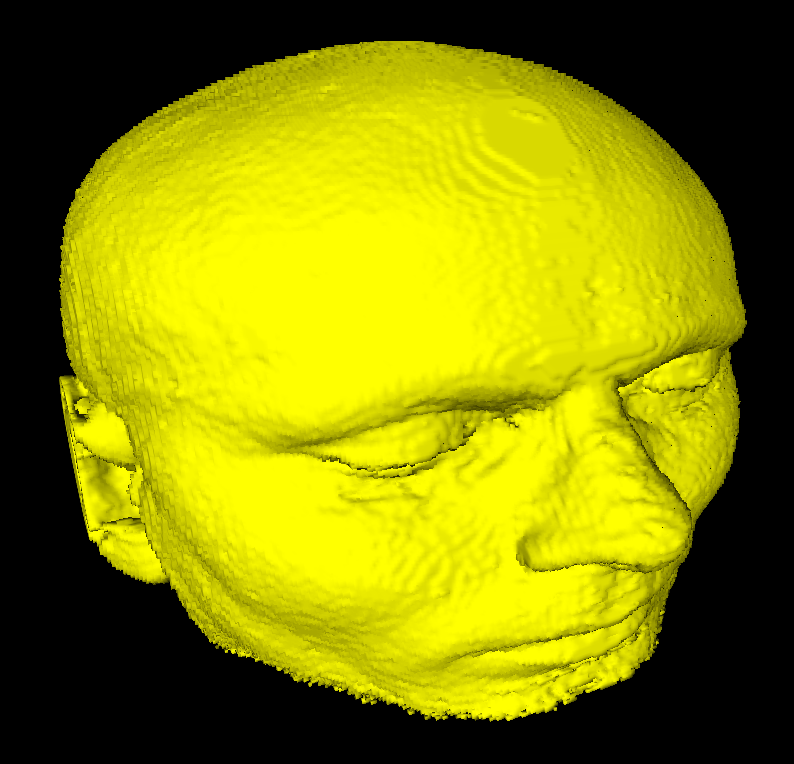
\includegraphics[scale=0.34]{img/cap03/MRI-Head-103-AZ-NS-BCC}}
  \end{center}
  \caption[Comparación visual en el modelo de una cabeza humana]{Comparación visual en el modelo de una cabeza humana.}
  \label{fig:MRI-Head}
\end{figure}

De esta figura es importante resaltar que aun cuando las mallas de Artzy (Figura \ref{fig:MRI-HeadAZ}) y MC (Figura \ref{fig:MRI-HeadMC}) producen resultados parecidos en las zonas de la nariz. Una vez que se hace el posprocesado, la misma zona se ve mucho mas suave en la Figura \ref{fig:MRI-HeadBCC}.

%Por último se muestran las mallas generadas a partir de datos de la reconstrucción de un cráneo humano. Este conjunto de datos es el mismo usado en las figuras \ref{fig:ejmploMC} y \ref{fig:ejmploArtzy} del primer capítulo pero visto desde otro punto de vista.

% \begin{figure}[htp]
%   \begin{center}
%     \subfigure[Malla de Artzy]{\label{fig:VisMaleAZ}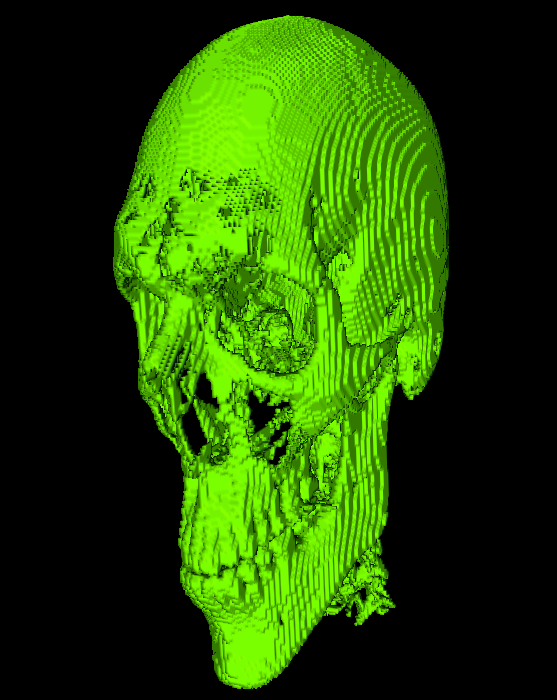
\includegraphics[scale=0.37]{img/cap03/VisMale-100-Az-BNS-AZ}}
%     \subfigure[Malla de MC]{\label{fig:VisMaleMC}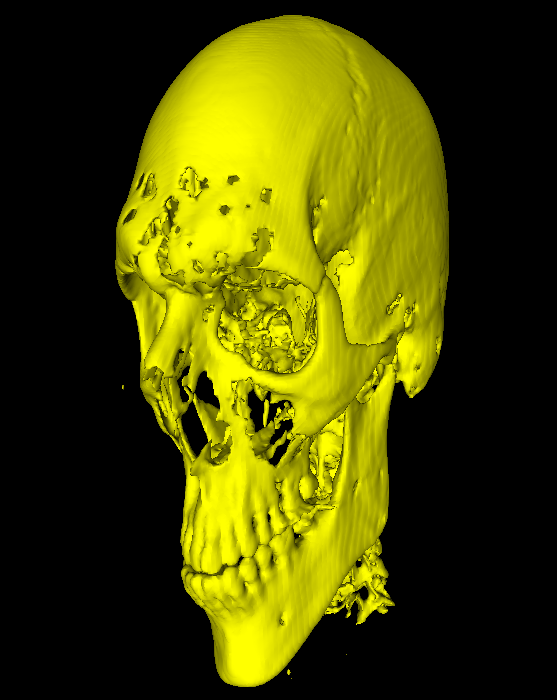
\includegraphics[scale=0.37]{img/cap03/VisMale-100-MC}} \\
%     \subfigure[Malla de Artzy con ponderación de normales caso \emph{sc}]{\label{fig:VisMaleSC}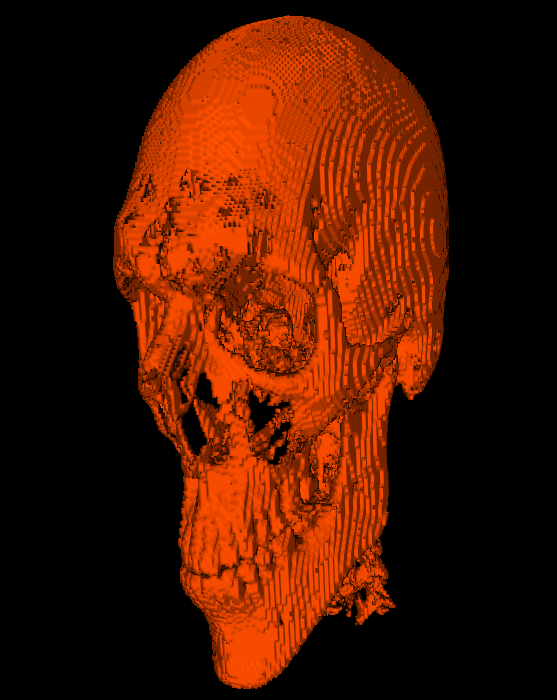
\includegraphics[scale=0.37]{img/cap03/VisMale-100-Az-BNS-SC}}
%     \subfigure[Malla de Artzy con ponderación de normales caso \emph{bcc}]{\label{fig:VisMaleBCC}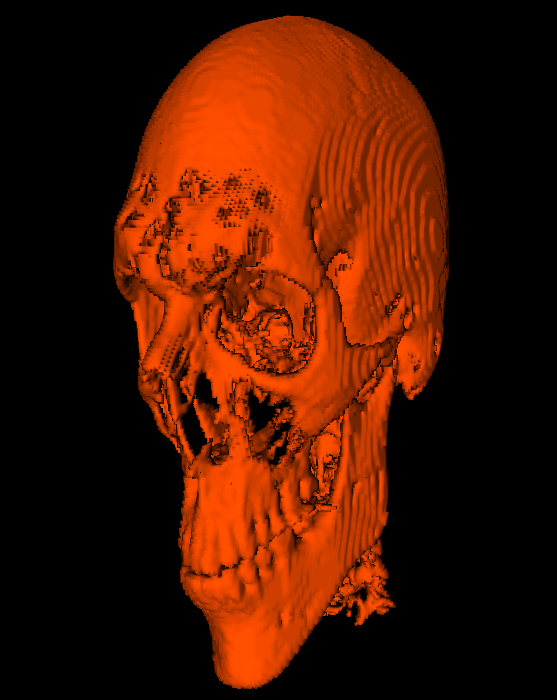
\includegraphics[scale=0.37]{img/cap03/VisMale-100-Az-BNS-BCC}}
%   \end{center}
%   \caption[Comparación visual de mallas generadas a partir de datos de reconstrucción de una cabeza humana]{Comparación visual de mallas generadas a partir de datos de reconstrucción de una cabeza humana.}
%   \label{fig:VisMale}
% \end{figure}

%En la figura \ref{fig:VisMale} se pueden apreciar áreas muy homogéneas y áreas con mas detalle. Por ejemplo áreas cercanas a la frente del cráneo, donde se aprecia que la ponderación suavizo muy poco en \ref{fig:VisMaleBCC} con respecto a \ref{fig:VisMaleAZ} y no es tan suave como es la malla de MC. Sin embargo, en zonas de mediano detalle por ejemplo en la zona de los dientes el resultado de la ponderación de \emph{bcc}, es comparable con MC, aun cuando esta ocupando la misma malla de Arzy.

\section{Experimentos con maniquíes (\emph{phantoms})}
\label{sec:experimentosMaquetas}

En los experimentos realizados en la sección anterior no se conoce la función original y por lo tanto es difícil realizar una comparación numérica, es por esta razón que diseñamos otros experimentos usando una función conocida la cual fue muestreada ``adecuadamente'' para generar la aproximación $v_{G_{\Delta}}$.

%En esta sección se describen experimentos realizados sobre reconstrucciones a partir de descripciones geométricas. Para hacer esas reconstrucciones se uso el método de ART . Como parte del SW disponible es posible modificar la distancia de muestreo $\Delta$ y por lo tanto producir varias aproximaciones a diferente resolución del conjunto $v$.
Para estos experimentos deseamos comparar nuestra aproximación con la ``realidad''. Como las superficies son diferentes y solo modificamos las normales, realizamos la comparación de las normales del objeto real con las normales de nuestra aproximación.

\subsection{Medida de error}
Una medida de error de las normales puestas sobre la malla y las normales analíticas es el error medio de los ángulos entre esos vectores. Definido de la siguiente manera:

\begin{equation}
  \text{ME} = \sum \limits_{i = 1}^{m} \frac{|\arccos \left\langle \textbf{n}_{j}, \textbf{n}^{*}_{j} \right\rangle |}{m}.
  \label{ec:me}
\end{equation}
Con respecto a la ecuación \eqref{ec:me} cabe señalar que los vectores para iluminación son unitarios, por lo que $|\textbf{n}_{j}| = |\textbf{n}^{*}_{j}| = 1$ y por eso podemos calcular al ángulo por medio del producto punto.

En donde $\textbf{n}_{j}$ es la normal analítica de la superficie $S_\tau$ y $\textbf{n}^{*}_{j}$ es la normal asignada en ese punto de la malla por el método de ponderado de normales.

\subsection{Criterio de muestro}

Para este análisis se usa como base una esfera unitaria que forma un campo escalar de densidad uniforme y también unitaria, es decir: 

\begin{equation}
  s(\textbf{x}) = 
    \begin{cases} 
      1, & \text{ si } |\textbf{x}| \leq 1, \\
      0, & \text{ en otro caso.} \\                                
    \end{cases}
\label{ec:sphere}
\end{equation}

Se sabe que la transformada de Fourier de esa función esta dada por la siguiente expresión \cite{fourierBook}

\begin{equation}
  \hat{s}(\bm \xi) = \dfrac{J_1 (2 \pi |\bm \xi|)}{\bm \xi}.
\label{ec:ftSphere}
\end{equation}
Sabemos también de \cite{fourierBook} que como la función es radialmente simétrica y su transformada también lo es podemos hacer el resto del análisis en una sola dimensión. Una forma de encontrar el valor de discretización es encontrar primero una frecuencia de corte de la transformada $\hat{f}$.

Un criterio razonable es cortar en los ceros de $\hat{s}$. Esta función es cero cuando el numerador es cero, por lo tanto podemos buscar los valores $u$ para los cuales

\begin{eqnarray}
  \nonumber
  J_1(2 \pi \xi) & = & 0, \\
  \nonumber
  2 \pi \xi & = & u, \\
  \xi & = & \frac{u}{2 \pi}.
  \label{ec:frecCorte}
\end{eqnarray}
la función $J_1$ tiene varios valores $u$ tales que $J_1(u) = 0$, su gráfica puede verse en la Figura \ref{fig:grafBess1}. Numéricamente se determinaron los primeros cinco valores $u$ para los que $J_1(u)=0$. Luego para cada uno de ellos se determinó un valor en el espacio de Fourier con \eqref{ec:frecCorte} que se tomo como frecuencia de corte. 

\begin{figure}[htp]
 \centering
  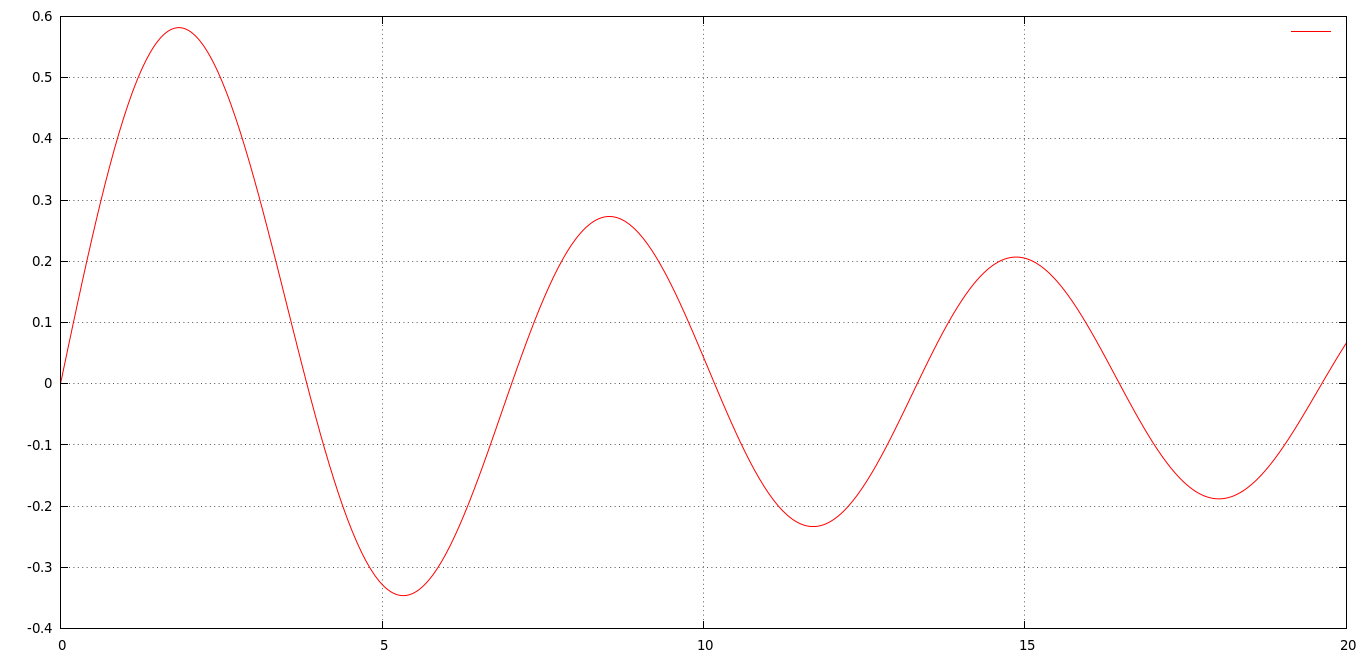
\includegraphics[scale=0.3]{img/cap03/J_1}
  \caption[Gráfica de la función $J_{1}$ en la frecuencia]{Gráfica de la función $J_{1}$ en la frecuencia.}
  \label{fig:grafBess1}
\end{figure}

Una vez calculada la frecuencia de corte $\xi$, el ancho de banda es $2 \xi$, como en el espacio de Fourier las magnitudes son inversas al espacio real entonces $\frac{1}{2 \xi}$ es la distancia de muestro $\Delta$ para cada caso.

\begin{table}[htp]
\begin{center}
  \begin{tabular}{|r|r|r|r|}
    \hline
    Valor de $u$ & Frecuencia de corte $\xi$ & Distancia de muestreo $\Delta$ & Número de vóxeles \\ 
    \hline
     3.83 & 0.61 & 32.79 &  4 \\
     7.01 & 1.12 & 17.91 &  7 \\
    10.17 & 1.62 & 12.35 & 10 \\
    13.32 & 2.12 &  9.43 & 14 \\
    16.47 & 2.62 &  7.62 & 17 \\
    \hline
  \end{tabular}
\end{center}
\caption[Discretizaciones correspondientes para distintos ceros de la función $J_{1}(\xi)$]{En esta tabla se muestran las discretizaciones correspondientes para distintos ceros de la función $J_{1}(\xi)$.}
\label{table:anaFourier}
\end{table}

La reconstrucción fue muestreada a cada una de estas discretizaciones. Finalmente, a cada superficie se le aplica el ponderado de normales y se mide su error medio.

A cada una de las normales asignadas $\textbf{n}_j$ se mide su error con respecto a la normal en la superficie de la esfera. Sin embargo, debido a que $\mathcal{A}_{\tau}$ es una aproximación a $S_{\tau}$ es muy posible que los vértices de la malla $\mathcal{A}_{\tau}$ no estén sobre la superficie analítica de la esfera. Para poder hacer la comparación si un vértice $\textbf{p}$ de la malla $\mathcal{A}_{\tau}$ no esta en la superficie es proyectado a un punto de la superficie y luego se mide el error de su normal con respecto a la del punto donde fue proyectado, esto se ve en la Figura \ref{fig:nomalesProy}. Puede ser que tenga que ser proyectado hacia afuera si originalmente estaba dentro de la superficie, Figura \ref{fig:normDentro}, o que tenga que ser proyectado hacia adentro si originalmente estaba fuera de la superficie, como en la Figura \ref{fig:normFuera}.

\begin{figure}[htp]
  \begin{center}
    \subfigure[El punto de la malla esta dentro de la esfera.]{\label{fig:normDentro}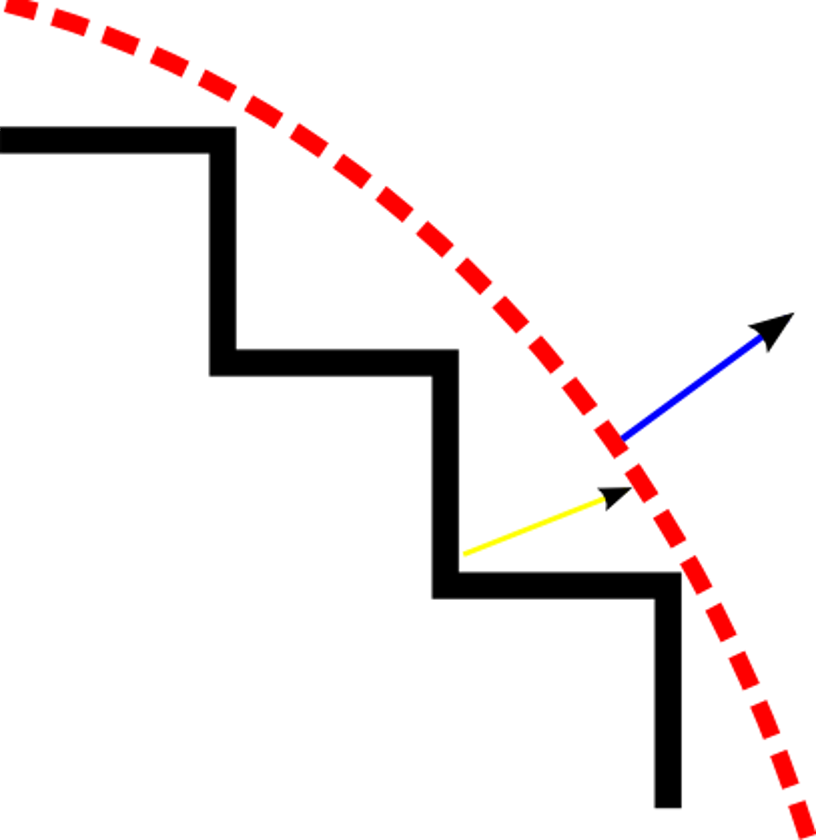
\includegraphics[scale=1]{img/cap03/normales1}}
    \hspace{8mm}
    \subfigure[El punto de la malla queda fuera de la esfera.]{\label{fig:normFuera}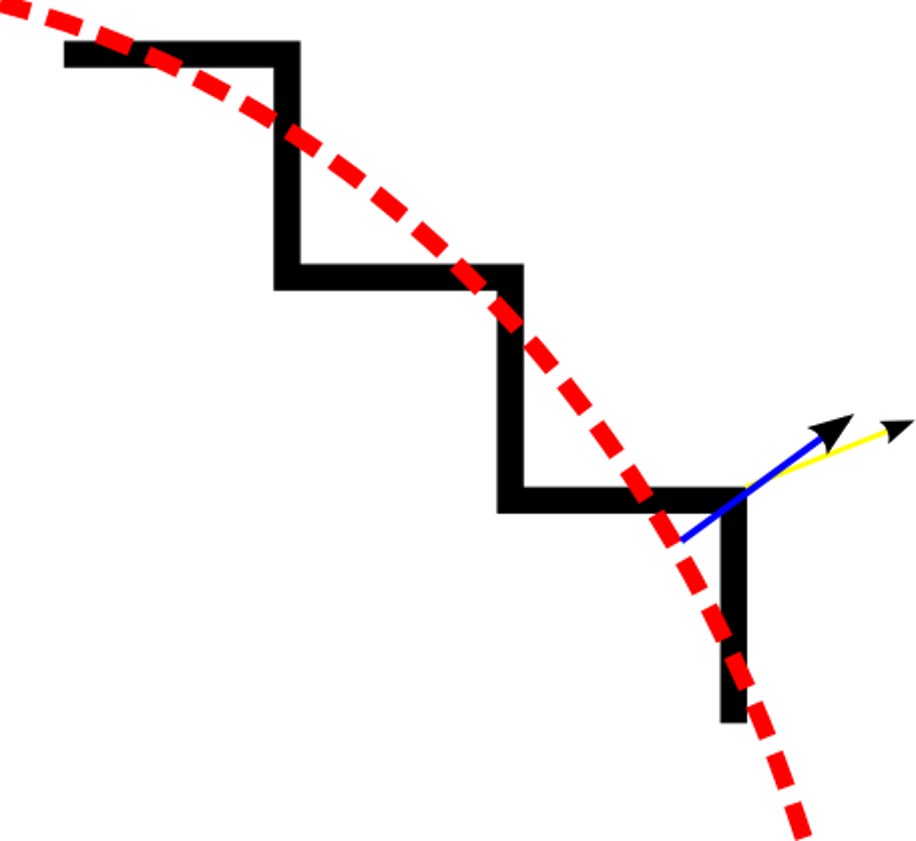
\includegraphics[scale=1]{img/cap03/normales2}} \\
  \end{center}
  \caption[Esquema para la comparación de normales en la superficie de la esfera]{Esquema para la comparación de normales en la superficie de la esfera. La malla se muestra en negro, la superficie de la esfera en rojo con lineas punteadas. La normal asignada con la ponderación es el vector amarillo, la normal contra la cual se compara es el vector en azul.}
  \label{fig:nomalesProy}
\end{figure}

Los resultados del experimento se resumen el la Tabla \ref{table:esfera}. En la segunda columna se muestra el ángulo de mayor error medido en radianes. La tercera columna tiene el error medio medido en grados.

\begin{table}[htp]
\begin{center}
  \begin{tabular}{|r|r|r|r|}
    \hline
    Discretización & Ángulo de mayor error & ME en grados\\ 
    \hline
      4 & 0.00049 & 0.10 \\
      7 & 0.02561 & 0.75 \\
     10 & 0.06333 & 2.23 \\
     14 & 0.18293 & 4.43 \\
     17 & 0.18766 & 4.03 \\
    \hline
  \end{tabular}
\end{center}
\caption[Resultados del experimento numérico sobre una esfera]{Resultados del experimento numérico sobre una esfera.}
\label{table:esfera}
\end{table}

De la tabla anterior podemos apreciar que en el error es muy pequeño y parece aumentar conforme la discretización de la esfera aumenta hasta un cierto umbral en donde empieza a disminuir.

Aunque el experimento es numérico se consideró prudente, en el caso de la esfera, mostrar la imagen de dos realizaciones del experimento. En la Figura \ref{fig:nomalesEsfera} se muestra en el lado izquierdo la malla de Arzty y en el lado derecho la malla con el ponderado de normales. En las dos primeras imágenes se muestra para una escena de 10 vóxeles de tamaño y en el segundo renglón para una escena de tamaño de 17 vóxeles.

\begin{figure}[htp]
  \begin{center}
    \subfigure[Malla de Artzy. Escena de 10 voxeles]{\label{fig:Az-10}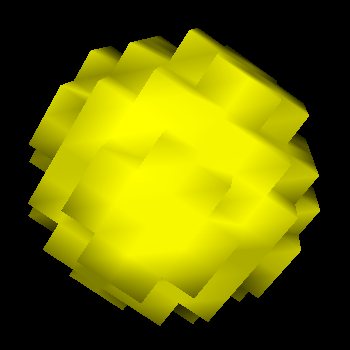
\includegraphics[scale=0.77]{img/cap03/Az10}}
    \subfigure[Malla con normales ponderadas. Escena de 10 voxeles]{\label{fig:Az-10-NS}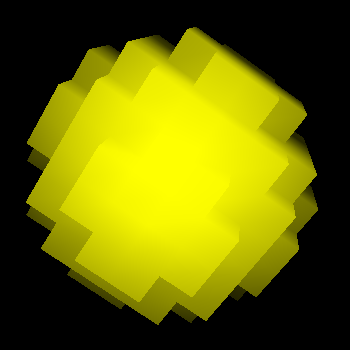
\includegraphics[scale=0.77]{img/cap03/Az10-NS}} \\
    \subfigure[Malla de Artzy. Escena de 17 voxeles]{\label{fig:Az-17}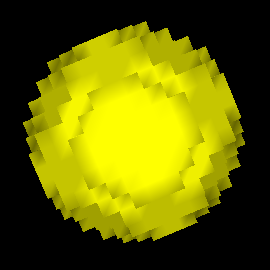
\includegraphics[scale=1]{img/cap03/Az17}}
    \subfigure[Malla con normales ponderadas. Escena de 17 voxeles]{\label{fig:Az-17-NS}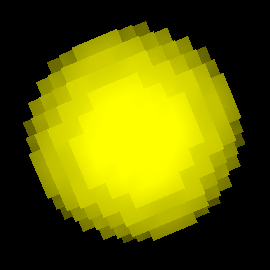
\includegraphics[scale=1]{img/cap03/Az17-NS}} \\
  \end{center}
  \caption[Resultados visuales de la ponderación de normales en el caso de la esfera]{Resultados visuales de la ponderación de normales en el caso de la esfera.}
  \label{fig:nomalesEsfera}
\end{figure}

Como los blobs son funciones esféricas se espera que se adapten mejor a la superficie de una esfera. Para poder hacer otra comparación se creo también un \emph{phantom} de un cubo cuyo lado mide lo mismo que el diámetro de la esfera en una escena del mismo tamaño. Para poder comparar el cubo con la esfera se realizaron las mismas discretizaciones.

Hay también que aclarar que la superficie $\mathcal{A}_{\tau}$ encontrada por el algoritmo de Artzy coincide totalmente con la superficie del phanthom del cubo. Por esta razón las normales de los vértices de la malla se comparan con las normales analíticas en el mismo punto. Los resultados se pueden ver en la Tabla \ref{table:cubo}.

\begin{table}[htp]
\begin{center}
  \begin{tabular}{|r|r|r|r|}
    \hline
    Discretización & Ángulo de mayor error & ME en grados\\ 
    \hline
      4 & 0.433081 & 13.51 \\
      7 & 0.433081 & 11.88 \\
     10 & 0.433081 &  8.18 \\
     14 & 0.433081 &  5.72 \\
     17 & 0.433081 &  5.32 \\
    \hline
  \end{tabular}
\end{center}
\caption[Resultados del experimento numérico sobre un cubo]{Resultados del experimento numérico sobre un cubo.}
\label{table:cubo}
\end{table}

En este experimento llama la atención que el blob parece no adaptarse tan finamente como en el caso de la esfera pues el error promedio es considerablemente mayor que en el modelo anterior. También es de llamar la atención que el caso de mayor error se mantiene constante.

%El primer modelo es una esfera centrada en el origen de radio $40$ en una escena de tamaño $128$. Este modelo fue muestreado con un $\Delta = \frac{1}{2}$. Después se calculo el volumen analítico de la esfera y se escogió el isovalor que hace el volumen de la isosuperficie de la esfera mas cercano al valor real, con eso se genero una malla $\mathcal{A}_{\tau}$. 
